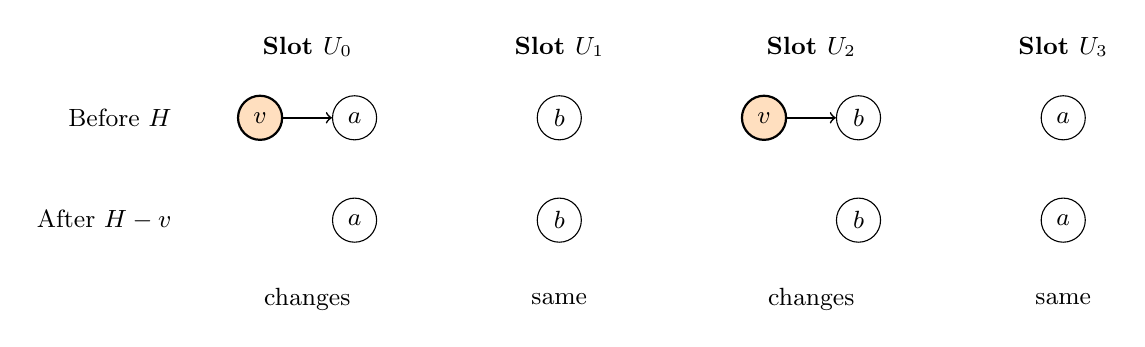
\begin{tikzpicture}[
  font=\small, x=1mm, y=1mm,
  vertex/.style={circle, draw, inner sep=1pt, minimum size=5.6mm, fill=white},
  removed/.style={vertex, thick, fill=orange!25},
  edge/.style={semithick, ->}
]
\foreach \x/\slot/\name in {0/0/changes,32/1/same,64/2/changes,96/3/same} {
  \node[font=\small\bfseries] at (\x,0) {Slot \(U_{\slot}\)};
  \node at (\x,-32) {\name};
}
\node[anchor=east] at (-16,-9) {Before \(H\)};
\node[anchor=east] at (-16,-22) {After \(H-v\)};

\node[removed] (v0) at (-6,-9) {\(v\)};
\node[vertex] (a0) at (6,-9) {\(a\)};
\draw[edge] (v0) -- (a0);
\node[vertex] at (6,-22) {\(a\)};

\foreach \y in {-9,-22} {
  \node[vertex] at (32,\y) {\(b\)};
  \node[vertex] at (96,\y) {\(a\)};
}

\node[removed] (v2) at (58,-9) {\(v\)};
\node[vertex] (b2) at (70,-9) {\(b\)};
\draw[edge] (v2) -- (b2);
\node[vertex] at (70,-22) {\(b\)};
\end{tikzpicture}
